\chapter{Experiments and Results}
\label{ch:results}

All numbers in this chapter are produced by notebooks 03--07 and stored in
\texttt{results/metrics}. Unless stated otherwise, results are mean $\pm$ standard deviation over three
seeds, and Daphnet inputs are normalised with independent, label-free domain statistics.

\section{Model selection on a saturated source task}
\label{sec:selection}

The first surprise came before any transfer experiment. With impact-centred labels, fall detection
on SisFall is close to solved: 18 of the 24 configurations in the search reach a validation AUPRC of
at least 0.999, and the selected models of every architecture reach 1.000 within two or three epochs (\Cref{fig:curves},
\Cref{fig:hpsearch}). AUPRC therefore cannot rank configurations or checkpoints, so we break ties with
the unweighted validation cross-entropy, which keeps decreasing for several more epochs. The selected
models are listed in \Cref{tab:hparams}. The search picked a two-layer bidirectional network for both
recurrent families, and the GRU ended up with the smallest model of the four (26k parameters).

\begin{table}[ht]
\centering
\small
\caption{Configurations selected on SisFall validation, trainable parameters, mean epochs to the selected checkpoint and training time per epoch on one NVIDIA T4 GPU.}
\label{tab:hparams}
\begin{adjustbox}{max width=\textwidth}
\begin{tabular}{lp{6.3cm}rrrr}
\toprule
Model & Configuration & lr & Params & Best ep. & s/epoch \\
\midrule
CNN-1D & width 32, kernel 7, dropout 0.5 & 3e-3 & 36,289 & 5.7 & 2 \\
LSTM & hidden 64, 2 layers, bidirectional, dropout 0.3 & 1e-3 & 135,425 & 8.0 & 4 \\
GRU & hidden 32, 2 layers, bidirectional, dropout 0.1 & 3e-3 & 26,241 & 9.7 & 2 \\
Transformer & $d=64$, 2 layers, patch 8, dropout 0.2 & 3e-3 & 70,401 & 7.3 & 3 \\
\bottomrule
\end{tabular}
\end{adjustbox}
\end{table}

Among the 18 saturated configurations, Daphnet AUROC ranges from 0.43 to 0.69 and is unrelated to
validation AUPRC (Spearman $\rho=0.23$, $p=0.37$). It is moderately related to validation loss
($\rho=-0.49$, $p=0.04$): better-calibrated source models transfer slightly better, which supports the
tie-breaking rule but is far from a reliable selection signal. An oracle that picked the
configuration with the best Daphnet AUROC would have changed the choice for the CNN only (0.54 $\to$
0.69 in the search setting) and for the LSTM marginally (0.51 $\to$ 0.52). We do not use these oracle
choices anywhere else.

\section{E1: in-domain fall detection}
\label{sec:e1}

\Cref{tab:sisfall} and the left panels of \Cref{fig:roc} report results on the eight held-out SisFall
subjects (381 fall windows, 14{,}173 non-fall windows, i.e.\ 3.9 hours of activity). The four
architectures are within two points of each other on every metric. The recurrent models have the
highest AUROC (0.999) and the fewest false alarms (0.7--0.8 per hour of activity). The CNN-1D has the
highest recall (0.980) but a lower AUROC (0.987), caused by a handful of falls that receive very low
scores; its seed-to-seed variability is also the largest (thresholds selected on validation range from
0.12 to 0.94). The Transformer misses the most falls (recall 0.959, about 16 of 381 per seed against 8
for the recurrent models). Subject-level bootstrap intervals overlap for all models (\Cref{tab:ci}).
In short, on the source task all four architectures are excellent, and the data do not support
ranking them.

\begin{table}[ht]
\centering
\footnotesize
\caption{In-domain fall detection on the eight SisFall test subjects (mean $\pm$ std over three seeds). Recall, specificity, F$_1$ and false alarms per hour (FA/h, one negative window per second of activity) use the threshold selected on validation. Best mean in bold.}
\label{tab:sisfall}
\setlength{\tabcolsep}{4pt}
\begin{adjustbox}{max width=\textwidth}
\begin{tabular}{lcccccc}
\toprule
Model & AUROC & AUPRC & Recall & Spec. & F$_1$ & FA/h \\
\midrule
CNN-1D & 0.987 $\pm$ 0.003 & 0.980 $\pm$ 0.002 & \textbf{0.980 $\pm$ 0.002} & \textbf{1.000 $\pm$ 0.000} & 0.982 $\pm$ 0.006 & 1.5 $\pm$ 1.1 \\
LSTM & \textbf{0.999 $\pm$ 0.000} & 0.990 $\pm$ 0.002 & 0.977 $\pm$ 0.010 & \textbf{1.000 $\pm$ 0.000} & \textbf{0.985 $\pm$ 0.005} & 0.8 $\pm$ 0.0 \\
GRU & \textbf{0.999 $\pm$ 0.000} & \textbf{0.992 $\pm$ 0.002} & 0.977 $\pm$ 0.003 & \textbf{1.000 $\pm$ 0.000} & \textbf{0.985 $\pm$ 0.002} & \textbf{0.7 $\pm$ 0.1} \\
Transformer & 0.998 $\pm$ 0.001 & 0.984 $\pm$ 0.005 & 0.959 $\pm$ 0.010 & \textbf{1.000 $\pm$ 0.000} & 0.974 $\pm$ 0.008 & 0.9 $\pm$ 0.5 \\
\bottomrule
\end{tabular}
\end{adjustbox}
\end{table}

\begin{figure}[ht]
\centering
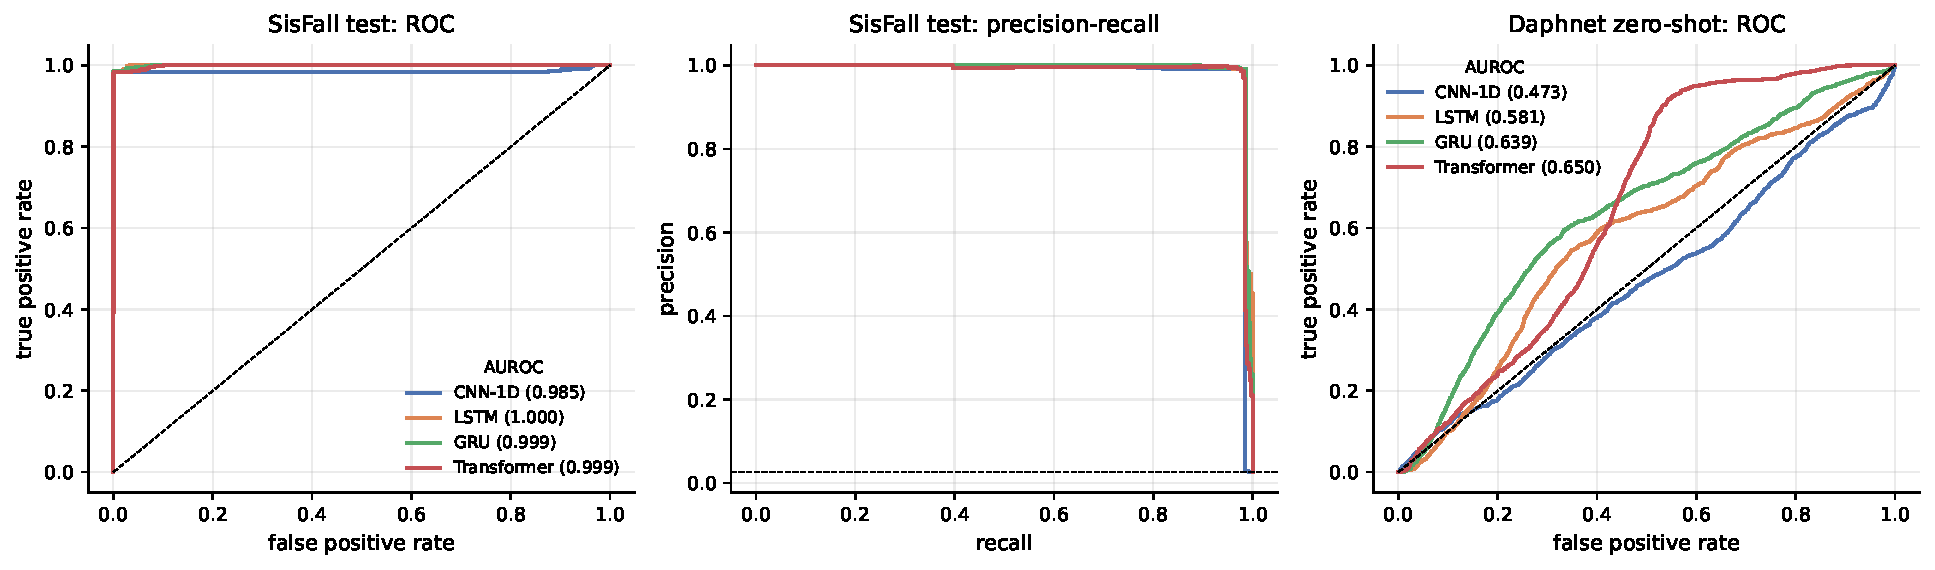
\includegraphics[width=\textwidth]{fig14_roc_pr_curves}
\caption{ROC and precision-recall curves of the seed-averaged scores. Left and centre: SisFall test
subjects. Right: zero-shot transfer to Daphnet.}
\label{fig:roc}
\end{figure}

\section{E2: zero-shot transfer to freezing of gait}
\label{sec:e2}

\paragraph{Ranking.} On Daphnet, AUROC falls to 0.49--0.63 (\Cref{tab:zeroshot}); AUPRC is 0.10--0.14
for a prevalence of 0.10. Averaging the three seeds gives 0.47 (CNN-1D), 0.58 (LSTM), 0.64 (GRU) and
0.65 (Transformer). With patients as the resampling unit, only the Transformer's 95\% interval excludes
chance, [0.55, 0.73] (\Cref{tab:ci}). The ROC curves (\Cref{fig:roc}, right) show that whatever
signal exists sits at mid-range false-positive rates, which is useless for an alarm.

\begin{table}[ht]
\centering
\footnotesize
\caption{Zero-shot transfer to Daphnet (all 17 recordings, independent domain statistics, SisFall-validated threshold). Positives are FoG windows. Best mean in bold.}
\label{tab:zeroshot}
\setlength{\tabcolsep}{4pt}
\begin{adjustbox}{max width=\textwidth}
\begin{tabular}{lcccccc}
\toprule
Model & AUROC & AUPRC & Recall & Spec. & F$_1$ & FA/h \\
\midrule
CNN-1D & 0.491 $\pm$ 0.056 & 0.104 $\pm$ 0.008 & \textbf{0.009 $\pm$ 0.008} & 0.994 $\pm$ 0.003 & \textbf{0.017 $\pm$ 0.015} & 23.3 $\pm$ 12.2 \\
LSTM & 0.587 $\pm$ 0.032 & 0.124 $\pm$ 0.021 & 0.001 $\pm$ 0.001 & 0.996 $\pm$ 0.000 & 0.001 $\pm$ 0.001 & 13.6 $\pm$ 0.9 \\
GRU & \textbf{0.631 $\pm$ 0.042} & \textbf{0.143 $\pm$ 0.023} & 0.000 $\pm$ 0.000 & \textbf{0.997 $\pm$ 0.001} & 0.000 $\pm$ 0.000 & \textbf{11.8 $\pm$ 5.1} \\
Transformer & 0.620 $\pm$ 0.036 & 0.128 $\pm$ 0.009 & 0.000 $\pm$ 0.000 & 0.995 $\pm$ 0.002 & 0.000 $\pm$ 0.001 & 17.1 $\pm$ 7.8 \\
\bottomrule
\end{tabular}
\end{adjustbox}
\end{table}
\begin{table}[ht]
\centering
\small
\caption{AUROC of the seed-averaged scores with 95\% subject-level bootstrap intervals.}
\label{tab:ci}
\begin{adjustbox}{max width=\textwidth}
\begin{tabular}{lcc}
\toprule
Model & SisFall test & Daphnet zero-shot \\
\midrule
CNN-1D & 0.985 [0.961, 1.000] & 0.473 [0.407, 0.546] \\
LSTM & 1.000 [0.999, 1.000] & 0.581 [0.381, 0.711] \\
GRU & 0.999 [0.998, 1.000] & 0.639 [0.458, 0.765] \\
Transformer & 0.999 [0.997, 1.000] & 0.650 [0.548, 0.733] \\
\bottomrule
\end{tabular}
\end{adjustbox}
\end{table}

\paragraph{Operating point.} At the threshold validated on SisFall, the detectors almost never fire on
Daphnet. Recall is below 1\% for every model, and the GRU flags none of the 1{,}734 FoG windows in any
seed (\Cref{fig:cm}). The score distributions explain why: walking and FoG windows both receive
log-odds between $-10$ and $-4$, four (CNN-1D) to ten (recurrent models, Transformer) units below the decision threshold (\Cref{fig:scores}).
This silence is informative in itself. With file-level labels, the pre-fall walking of SisFall
fall trials would be a positive example and irregular gait could easily look like a fall; with an
ankle sensor fed where the network expects a waist sensor, the inputs alone would push the scores up.
Either confounder could produce the opposite behaviour, an alarm on most Parkinsonian walking. Once
the event is defined as the impact and the sensors are matched, the detectors become very specific
to what they were taught.

\paragraph{False alarms still increase.} Even so, the false-positive rate on Daphnet walking is 0.3--0.7\%,
which corresponds to 12--23 false alarms per hour of walking, 15 to 18 times the rate measured on
healthy and elderly ADL. Covariate shift alone, without any FoG, degrades specificity by more than an
order of magnitude.

\begin{figure}[ht]
\centering
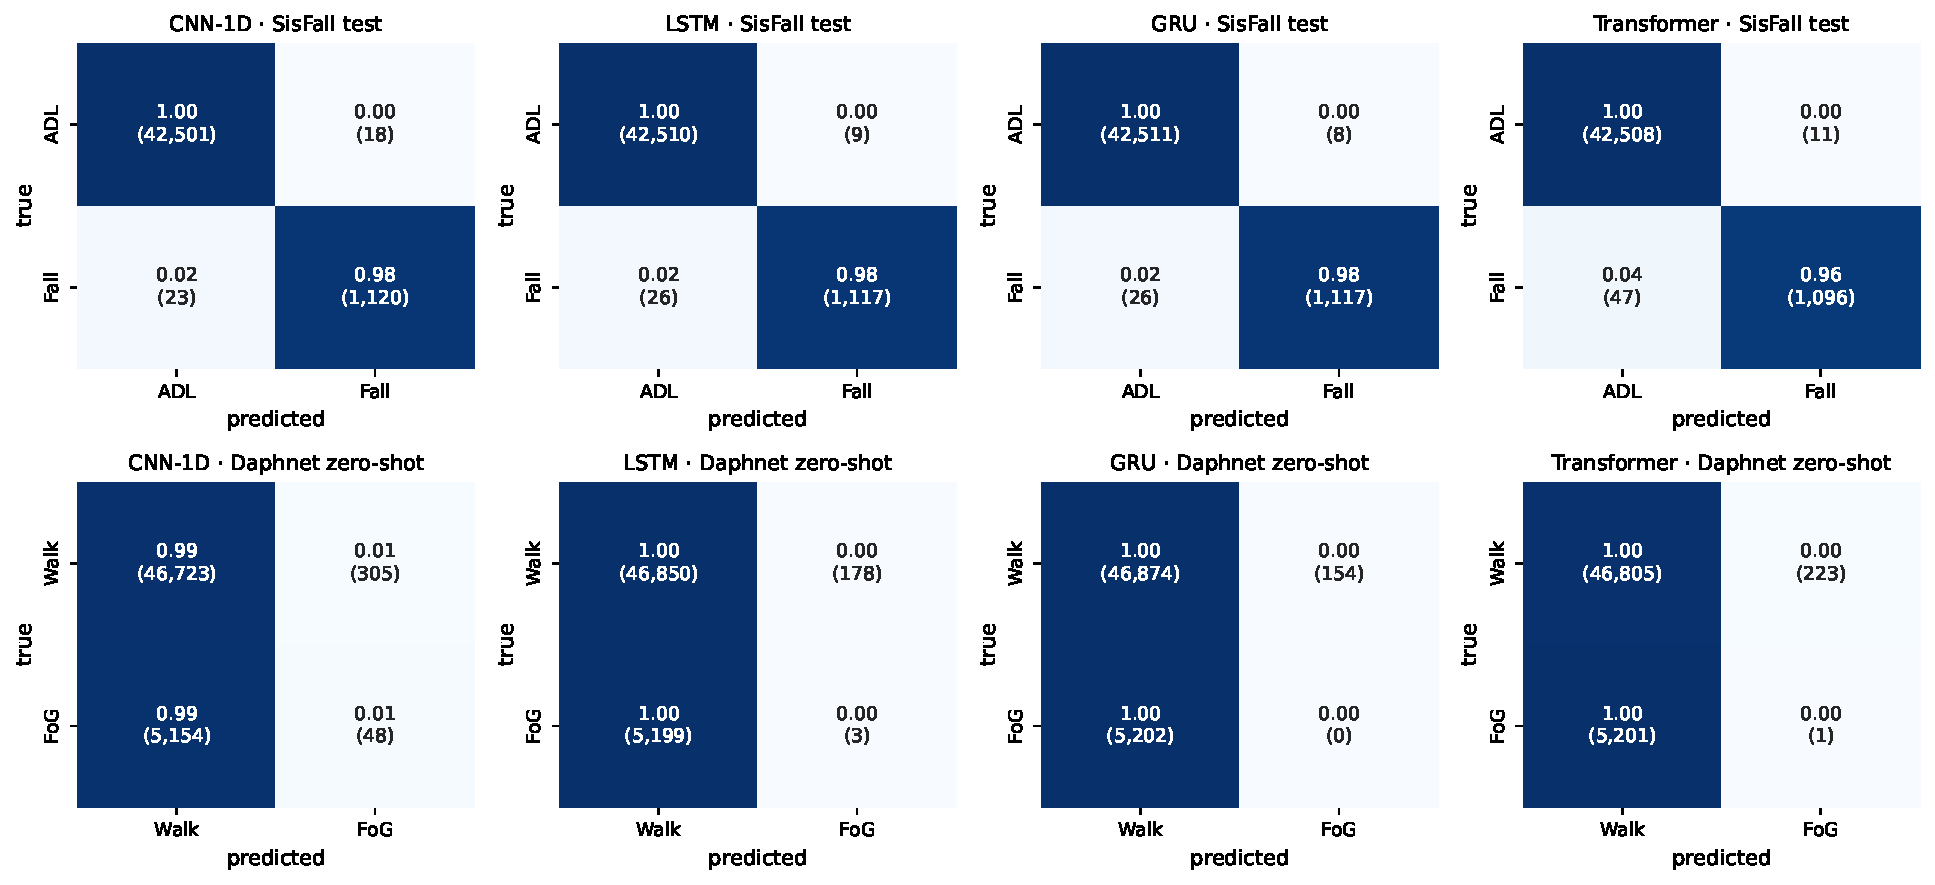
\includegraphics[width=\textwidth]{fig15_confusion_matrices}
\caption{Confusion matrices summed over the three seeds. Top: SisFall test. Bottom: Daphnet zero-shot.
Rows are normalised; counts in brackets.}
\label{fig:cm}
\end{figure}

\begin{figure}[ht]
\centering
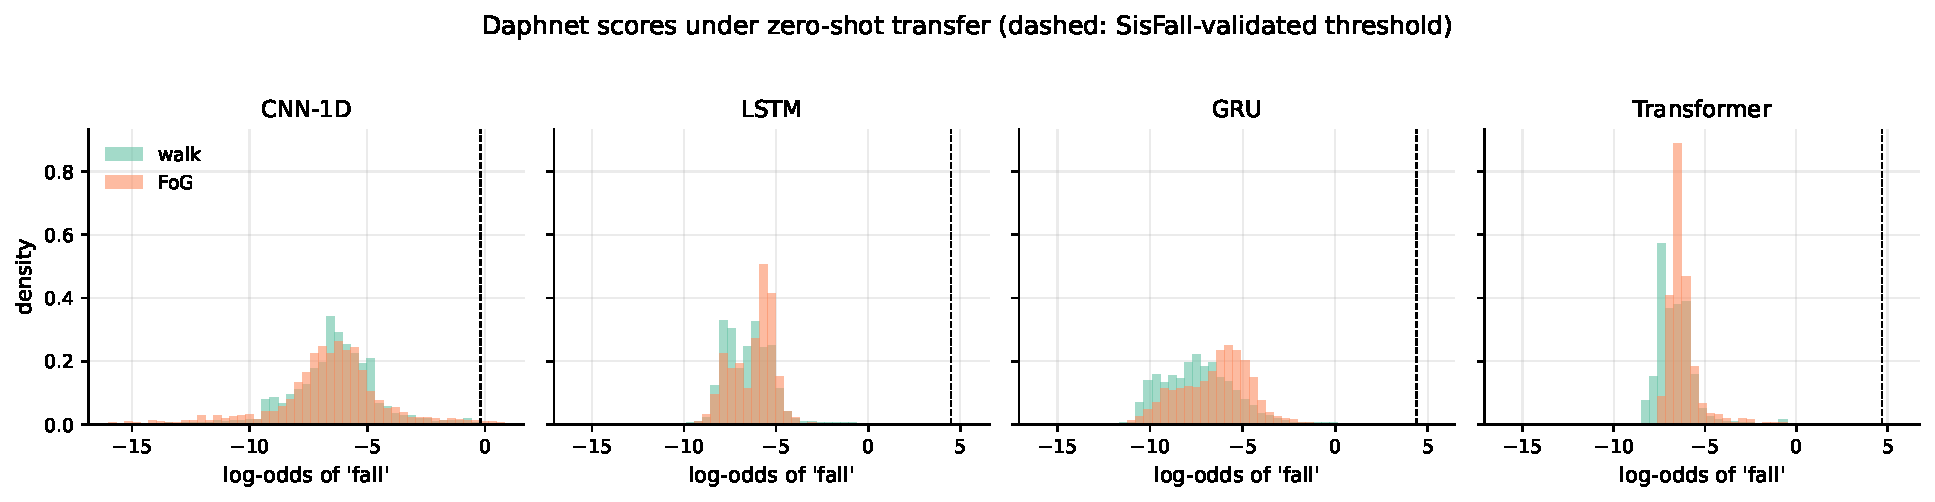
\includegraphics[width=\textwidth]{fig17_daphnet_score_distributions}
\caption{Seed-averaged Daphnet scores, shown as log-odds because almost all probabilities are close to
zero. The dashed line is the SisFall-validated threshold.}
\label{fig:scores}
\end{figure}

\paragraph{A training-free reference.} Two scores computed directly from each window, with no learning,
do better than every network: the freeze index on the trunk AP axis reaches an AUROC of 0.663, and
the standard deviation of $|a|$ reaches 0.682. At the trunk, FoG windows are on average more agitated
than the walking class, which also contains standing and turning. A fall detector could in principle
exploit that, but its scores carry less information about FoG than a single energy statistic.

\paragraph{Patients.} Per-patient AUROC ranges from 0.26 to 0.85 (\Cref{fig:perpatient}). The recurrent
models and the Transformer rank FoG above walking for S01, S02, S03 and S05 (0.60--0.85) and below it
for S06 and S08 (0.27--0.49). The CNN-1D shows almost the mirror pattern. A pooled AUROC around 0.6
thus hides patient-specific behaviour in both directions.

\begin{figure}[ht]
\centering
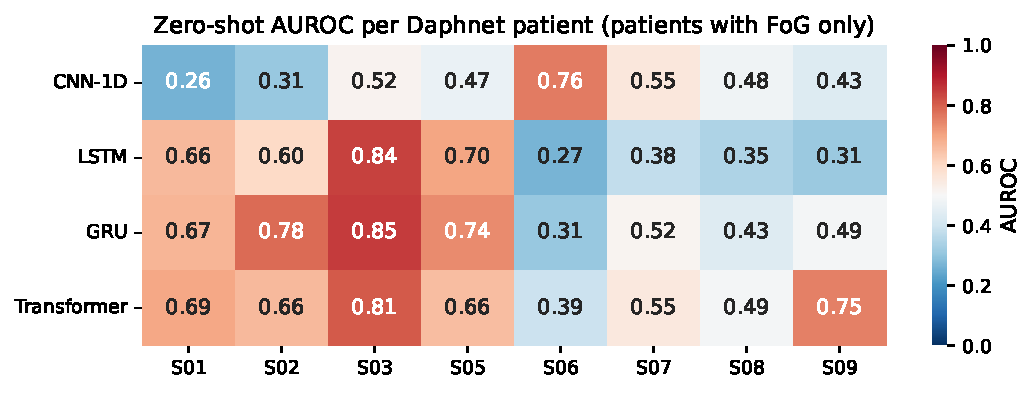
\includegraphics[width=0.9\textwidth]{fig18_per_patient_auroc}
\caption{Zero-shot AUROC per Daphnet patient (seed-averaged scores; S04 and S10 have no FoG).}
\label{fig:perpatient}
\end{figure}

\section{Does normalisation fix it?}
\label{sec:ablation}

\Cref{tab:ablation} and \Cref{fig:ablation} compare the three label-free normalisations of the target.
No variant brings any model close to the training-free reference. Re-estimating the statistics on
Daphnet helps the recurrent models and the Transformer slightly (GRU $+0.06$, LSTM $+0.04$, Transformer
$+0.02$) and hurts the CNN-1D ($-0.13$); per-patient statistics fall in between. First- and
second-order covariate correction at the input is not the bottleneck.

\begin{table}[ht]
\centering
\footnotesize
\caption{Zero-shot Daphnet results under three label-free normalisations of the target inputs: AUROC (mean $\pm$ std over seeds) and, in brackets, recall / false-positive rate at the SisFall threshold.}
\label{tab:ablation}
\begin{adjustbox}{max width=\textwidth}
\begin{tabular}{lccc}
\toprule
Model & Source statistics & Domain statistics & Subject statistics \\
\midrule
CNN-1D & 0.621 $\pm$ 0.064 (0.0\% / 0.2\%) & 0.491 $\pm$ 0.056 (0.9\% / 0.6\%) & 0.528 $\pm$ 0.042 (0.8\% / 2.0\%) \\
LSTM & 0.547 $\pm$ 0.064 (0.0\% / 0.1\%) & 0.587 $\pm$ 0.032 (0.1\% / 0.4\%) & 0.554 $\pm$ 0.031 (0.0\% / 0.4\%) \\
GRU & 0.571 $\pm$ 0.051 (0.0\% / 0.1\%) & 0.631 $\pm$ 0.042 (0.0\% / 0.3\%) & 0.604 $\pm$ 0.027 (0.0\% / 0.3\%) \\
Transformer & 0.603 $\pm$ 0.087 (0.0\% / 0.0\%) & 0.620 $\pm$ 0.036 (0.0\% / 0.5\%) & 0.596 $\pm$ 0.054 (0.0\% / 0.7\%) \\
\bottomrule
\end{tabular}
\end{adjustbox}
\end{table}

\begin{figure}[ht]
\centering
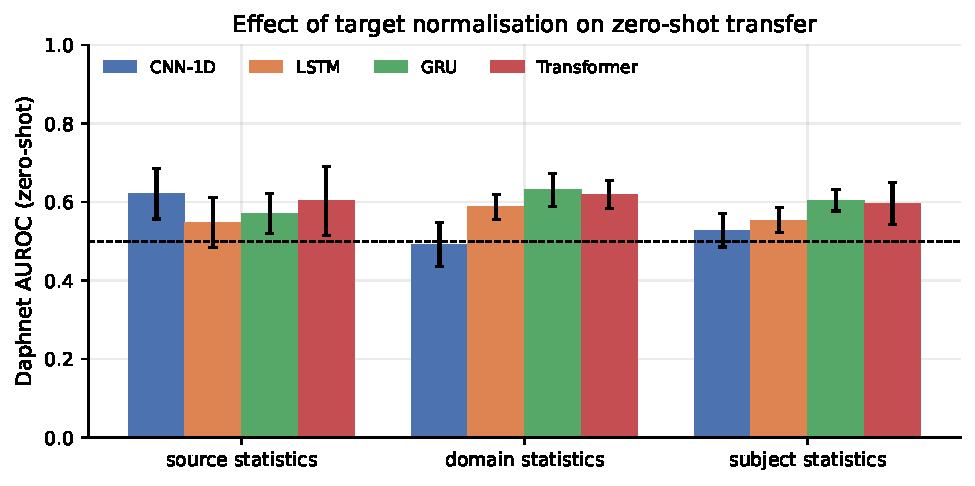
\includegraphics[width=0.75\textwidth]{fig13_normalisation_ablation}
\caption{Zero-shot Daphnet AUROC under three label-free normalisations (mean $\pm$ std over seeds).}
\label{fig:ablation}
\end{figure}

\section{E3: what target labels buy, and whether fall pre-training helps}
\label{sec:e3}

\Cref{tab:adaptation} and \Cref{fig:adaptation} give the target-domain references under 5-fold
patient-grouped cross-validation. Trained from scratch on six patients, the CNN-1D reaches an AUROC of
0.786, the Transformer 0.776 and the GRU 0.769, with large fold-to-fold variation ($\pm$0.15--0.19)
that reflects the heterogeneity between patients. The bidirectional LSTM is unstable with this little
data (0.608 $\pm$ 0.251). With only two training patients, the CNN-1D (0.714) and the Transformer
(0.696) degrade gracefully, while the recurrent models fall to chance. This trunk-only, 2\,s-window
ceiling of roughly 0.78 puts the zero-shot numbers in perspective: the best zero-shot model covers
about half of the distance between chance and this modest supervised ceiling, and the training-free
freeze index covers more.

\begin{table}[ht]
\centering
\footnotesize
\caption{Daphnet AUROC / AUPRC on held-out patients, 5-fold patient-grouped cross-validation (mean $\pm$ std over folds). FoG prevalence is 10\%, the AUPRC of a random detector.}
\label{tab:adaptation}
\setlength{\tabcolsep}{3pt}
\begin{adjustbox}{max width=\textwidth}
\begin{tabular}{lcccc}
\toprule
Setting & CNN-1D & LSTM & GRU & Transformer \\
\midrule
Zero-shot (no target labels) & 0.395$\pm$0.220 / 0.114 & 0.549$\pm$0.235 / 0.123 & 0.641$\pm$0.199 / 0.155 & 0.687$\pm$0.128 / 0.163 \\
Scratch, 2 patients & 0.714$\pm$0.123 / 0.238 & 0.351$\pm$0.256 / 0.104 & 0.548$\pm$0.255 / 0.195 & 0.696$\pm$0.153 / 0.215 \\
Fine-tuned, 2 patients & 0.617$\pm$0.144 / 0.161 & 0.435$\pm$0.170 / 0.089 & 0.588$\pm$0.167 / 0.132 & 0.668$\pm$0.195 / 0.179 \\
Scratch, 6 patients & 0.786$\pm$0.147 / 0.387 & 0.608$\pm$0.251 / 0.202 & 0.769$\pm$0.189 / 0.373 & 0.776$\pm$0.178 / 0.350 \\
Fine-tuned, 6 patients & 0.727$\pm$0.175 / 0.302 & 0.437$\pm$0.173 / 0.099 & 0.700$\pm$0.201 / 0.223 & 0.732$\pm$0.225 / 0.300 \\
\bottomrule
\end{tabular}
\end{adjustbox}
\end{table}

Fine-tuning from the SisFall weights does not help (\Cref{tab:pretrain}). With six training patients,
pre-training lowers the mean AUROC for all four architectures (by 0.04 to 0.17) and improves only one
fold out of five in each case. With two patients the picture is mixed (two small gains for the
recurrent models, two losses). None of the differences is significant with five folds (Wilcoxon
$p\geq0.125$), but the direction is consistent: the fall representation is a worse starting point
than random initialisation. This is negative transfer.

\begin{table}[ht]
\centering
\small
\caption{Effect of SisFall pre-training on Daphnet AUROC: mean difference (fine-tuned $-$ scratch), folds improved out of five, and Wilcoxon signed-rank $p$ (five folds, so $p\ge0.0625$).}
\label{tab:pretrain}
\begin{adjustbox}{max width=\textwidth}
\begin{tabular}{llrrrrr}
\toprule
Model & Budget & Scratch & Fine-tuned & $\Delta$ & Improved & $p$ \\
\midrule
CNN-1D & 2 patients & 0.714 & 0.617 & -0.097 & 1/5 & 0.312 \\
CNN-1D & 6 patients & 0.786 & 0.727 & -0.059 & 1/5 & 0.125 \\
LSTM & 2 patients & 0.351 & 0.435 & +0.083 & 3/5 & 0.438 \\
LSTM & 6 patients & 0.608 & 0.437 & -0.171 & 1/5 & 0.125 \\
GRU & 2 patients & 0.548 & 0.588 & +0.040 & 2/5 & 1.000 \\
GRU & 6 patients & 0.769 & 0.700 & -0.070 & 1/5 & 0.125 \\
Transformer & 2 patients & 0.696 & 0.668 & -0.028 & 2/5 & 0.625 \\
Transformer & 6 patients & 0.776 & 0.732 & -0.044 & 1/5 & 0.125 \\
\bottomrule
\end{tabular}
\end{adjustbox}
\end{table}

\begin{figure}[ht]
\centering
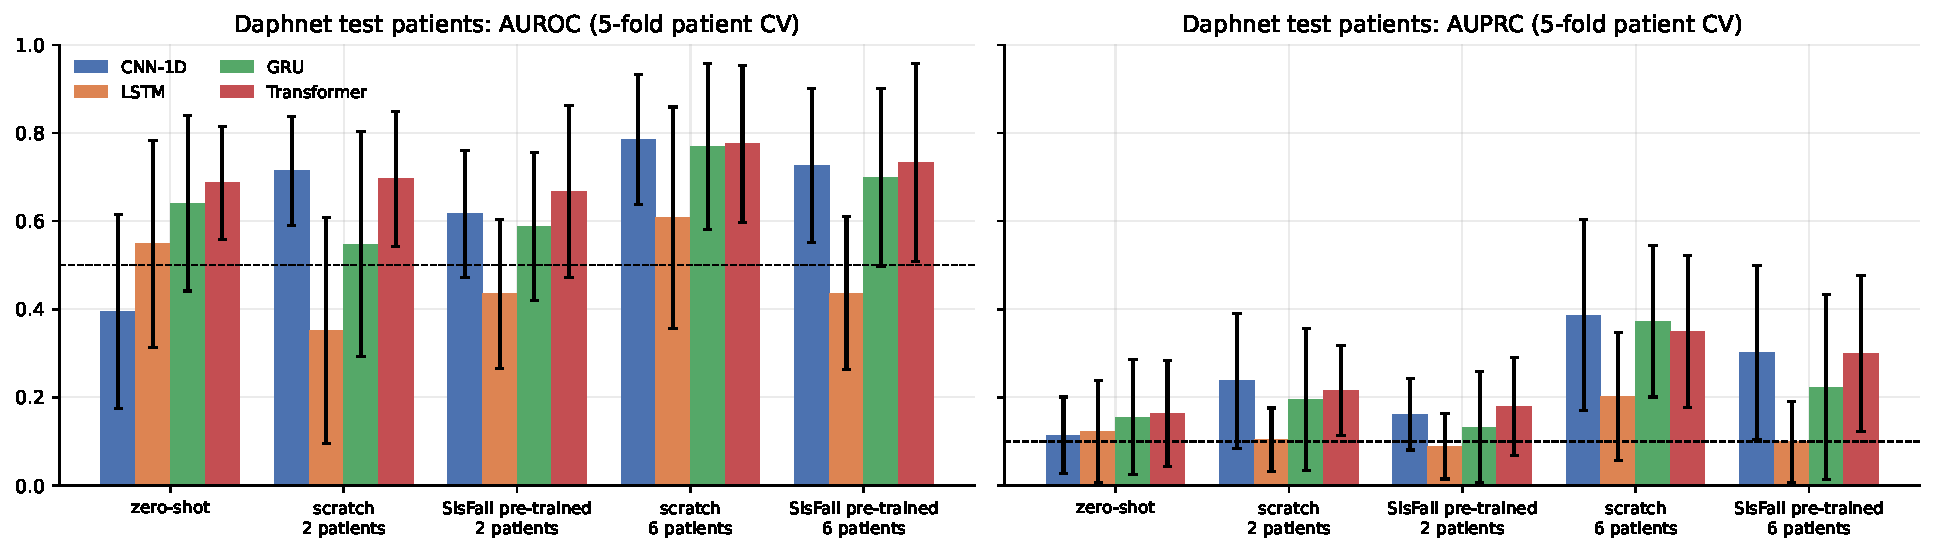
\includegraphics[width=\textwidth]{fig19_target_adaptation}
\caption{Daphnet AUROC and AUPRC on held-out patients (mean $\pm$ std over five folds). In the zero-shot
column the threshold is set on the validation patients of each fold, so its AUROC is computed on a
smaller set of patients than in \Cref{tab:zeroshot}.}
\label{fig:adaptation}
\end{figure}

\section{E4: covariate shift and concept shift in the representations}
\label{sec:e4}

\Cref{tab:shift} and \Cref{fig:shift} examine the penultimate-layer embeddings of the SisFall models
(seed 0).

\paragraph{Covariate shift is large and survives normalisation.} A linear probe separates SisFall ADL
from Daphnet walking with an AUROC of 0.96--0.995 in every space, whichever normalisation is used.
Domain statistics reduce the squared MMD considerably for the LSTM (0.446 $\to$ 0.017) and the
Transformer (0.128 $\to$ 0.024), but the probe accuracy hardly moves: matching moments is not the
same as making the domains indistinguishable. Parkinsonian walking remains recognisable as such
inside representations that were never trained to see it.

\paragraph{Concept shift is visible as orthogonality.} In raw window statistics, the vector from walking
to FoG points in the same direction as the vector from ADL to falls ($\cos=+0.77$): both mean ``more
movement''. In the learned embeddings, the cosine drops to $+0.18$ (CNN-1D), $+0.10$ (LSTM), $-0.03$
(GRU) and $+0.12$ (Transformer). The networks have learned features specific to impacts and discarded
the generic ``agitation'' direction, which is not discriminative on SisFall because jogging, stairs and
stumbling share it. That direction is precisely what distinguishes FoG from walking at the trunk. The
t-SNE maps (\Cref{fig:tsne-emb}) show the same picture: falls form a separate cluster, and Daphnet
walking and FoG windows are interleaved with each other and partly overlap SisFall ADL.

\begin{table}[ht]
\centering
\footnotesize
\caption{Shift between SisFall ADL and Daphnet walking, in input space and in the embedding of each SisFall-trained model: squared MMD, AUROC of a linear domain probe, under source and domain normalisation; and cosine between the fall and FoG class-difference directions.}
\label{tab:shift}
\setlength{\tabcolsep}{4pt}
\begin{adjustbox}{max width=\textwidth}
\begin{tabular}{lccccc}
\toprule
 & \multicolumn{2}{c}{MMD$^2$} & \multicolumn{2}{c}{Domain probe AUROC} & \\
\cmidrule(lr){2-3}\cmidrule(lr){4-5}
Space & source st. & domain st. & source st. & domain st. & $\cos(\Delta_\mathcal{S},\Delta_\mathcal{T})$ \\
\midrule
Input statistics & 0.110 & 0.072 & 0.958 & 0.995 & +0.766 \\
CNN-1D & 0.200 & 0.081 & 0.994 & 0.995 & +0.182 \\
LSTM & 0.446 & 0.017 & 0.989 & 0.975 & +0.096 \\
GRU & 0.097 & 0.074 & 0.993 & 0.981 & -0.030 \\
Transformer & 0.128 & 0.024 & 0.976 & 0.962 & +0.122 \\
\bottomrule
\end{tabular}
\end{adjustbox}
\end{table}

\begin{figure}[ht]
\centering
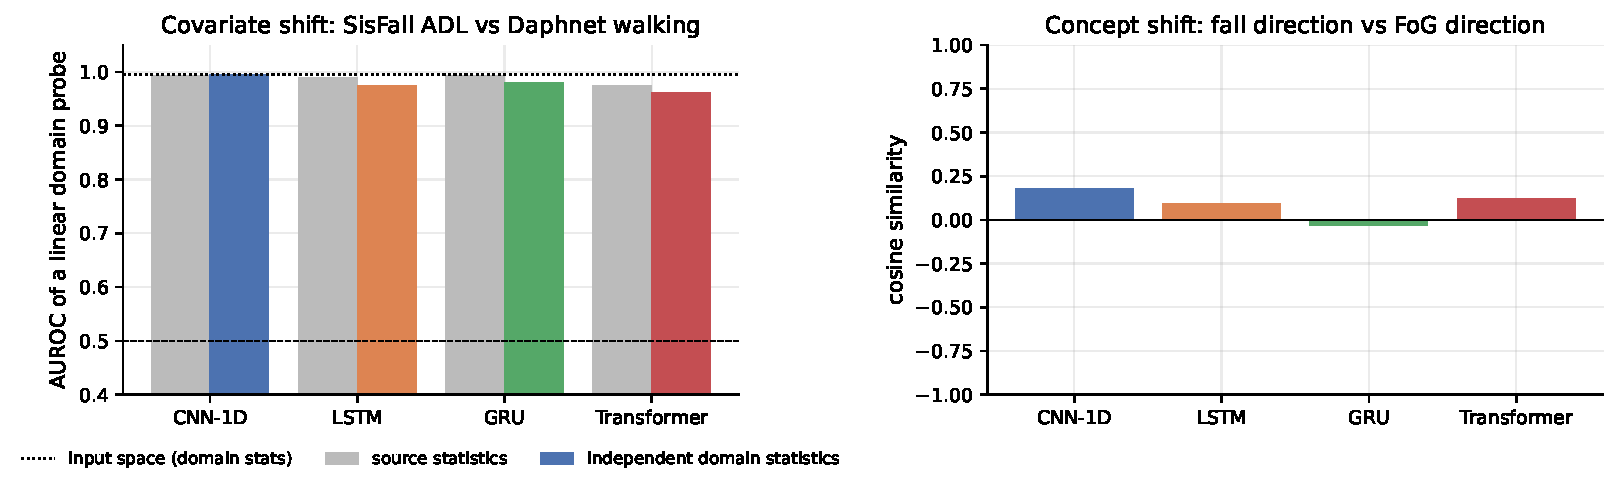
\includegraphics[width=\textwidth]{fig21_shift_decomposition}
\caption{Left: AUROC of a linear probe separating SisFall ADL from Daphnet walking in each model's
embedding (dotted line: input statistics). Right: cosine between the fall--ADL and FoG--walking
class-mean differences in each embedding.}
\label{fig:shift}
\end{figure}

\begin{figure}[ht]
\centering
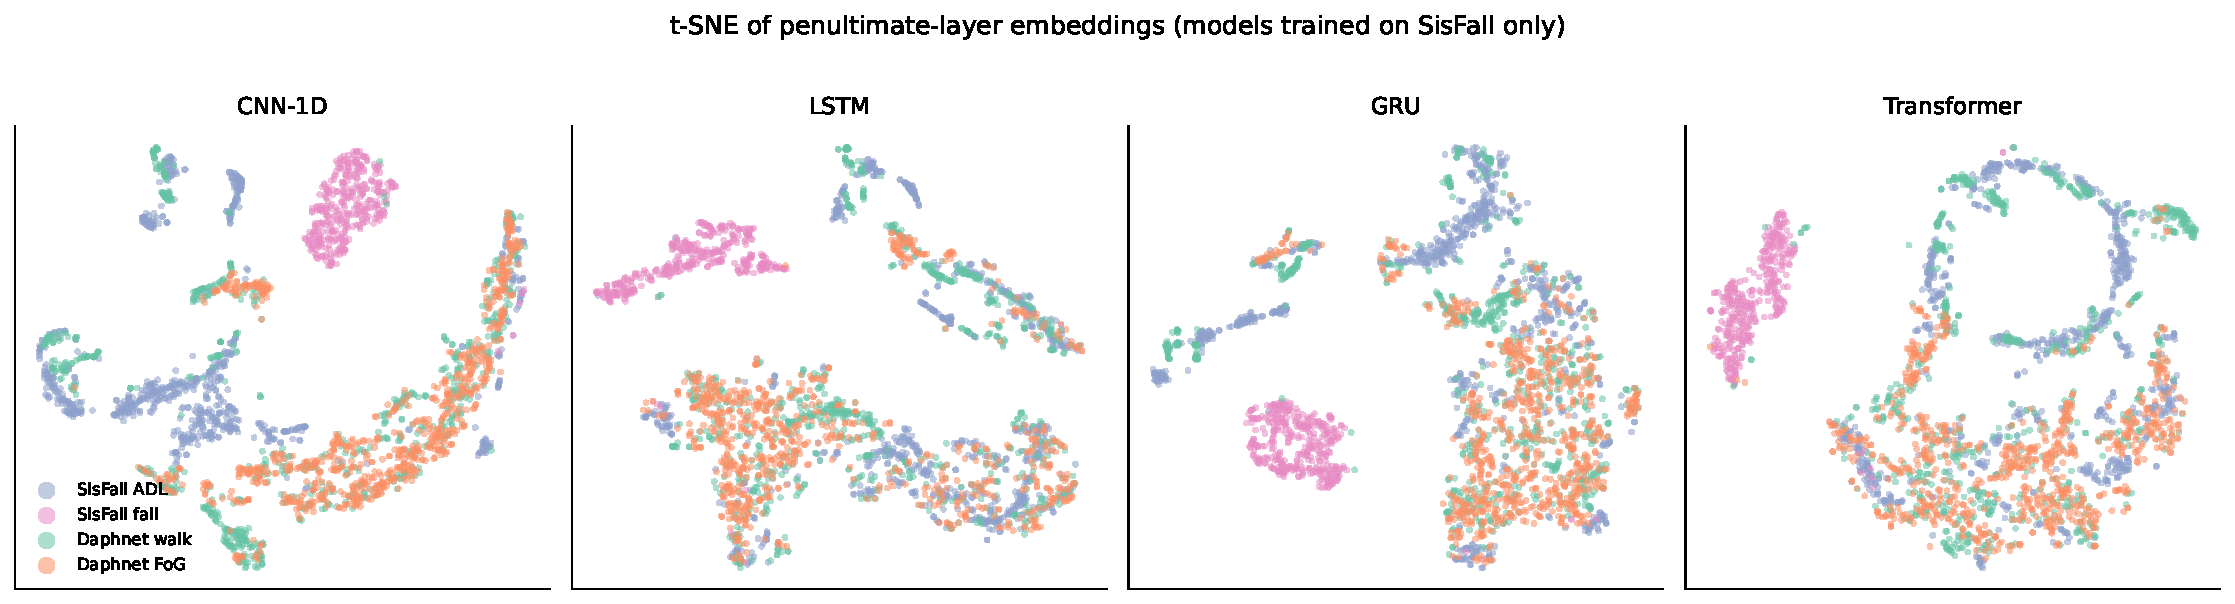
\includegraphics[width=\textwidth]{fig20_embedding_tsne}
\caption{t-SNE of penultimate-layer embeddings for 800 windows per group (SisFall test subjects and
Daphnet).}
\label{fig:tsne-emb}
\end{figure}

\section{Synthesis}
\label{sec:synthesis}

\Cref{fig:overview} gathers every setting. Four observations summarise the study.
\begin{enumerate}
  \item \textbf{In-domain accuracy says nothing about transfer.} All four models are near-perfect on
  SisFall and near chance on Daphnet. Source validation could not even rank configurations by
  transferability.
  \item \textbf{The failure is mostly concept shift.} Normalisation removes part of the covariate shift
  without improving transfer; the learned fall direction is orthogonal to the FoG direction; and fall
  pre-training hurts fine-tuning.
  \item \textbf{Architectures differ more under shift than in-domain, but not enough to matter.} The
  Transformer is the only model whose zero-shot interval excludes chance, and with the GRU it gives the
  best zero-shot ranking. The CNN-1D, worst under zero-shot transfer, is the best model once a few
  patients are labelled. None of these differences survives the patient-level uncertainty.
  \item \textbf{Physics beats transfer.} A 2008 hand-crafted freeze index, or simply the window's
  energy, ranks FoG better than any fall detector, without a single label.
\end{enumerate}

\begin{figure}[ht]
\centering
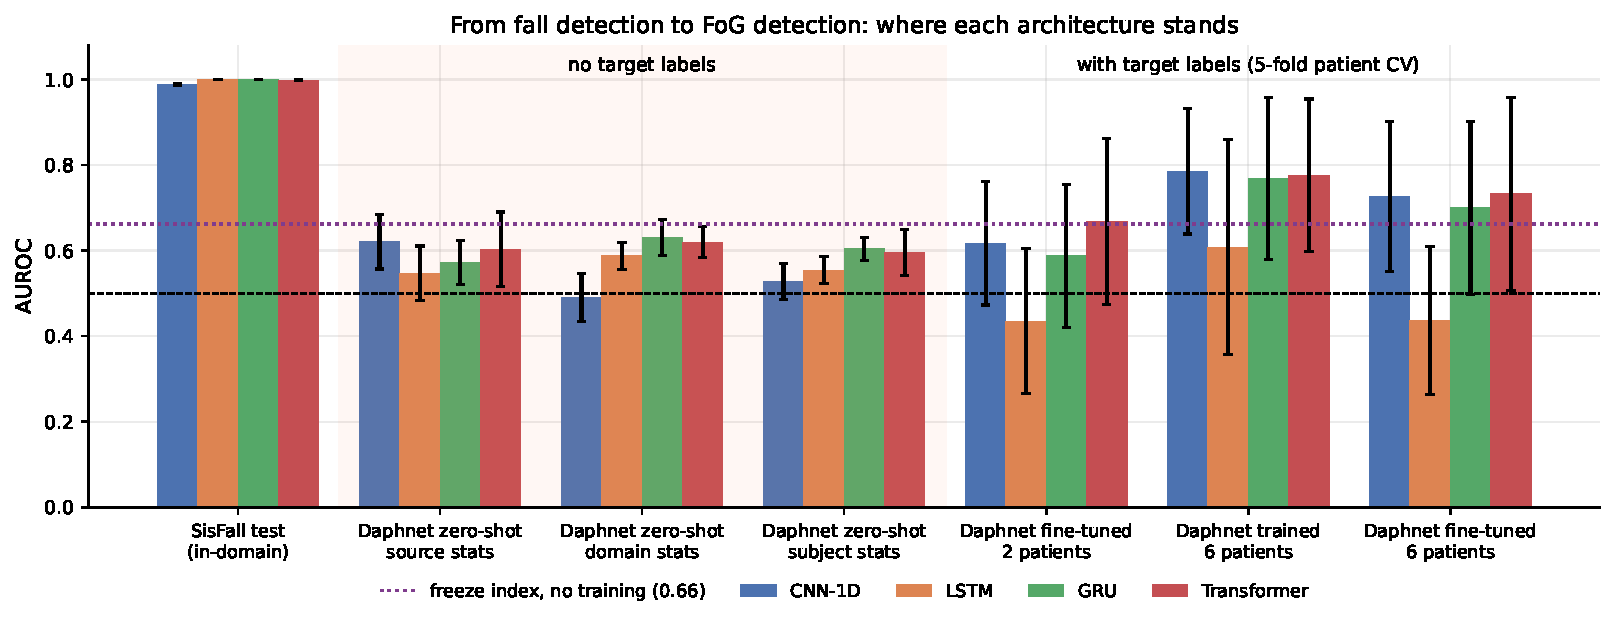
\includegraphics[width=\textwidth]{fig22_overview_auroc}
\caption{AUROC per setting and architecture (error bars: std over seeds for SisFall and zero-shot,
over folds for target-label settings). Dotted line: training-free freeze index.}
\label{fig:overview}
\end{figure}

\section{Limitations}
\label{sec:limitations}

Daphnet contains ten patients, two of whom never freeze, so every target-domain estimate carries wide
intervals; the subject bootstrap makes that explicit, but conclusions about architectures remain
tentative. The trunk sensor is the anatomically fair choice for comparison with SisFall, but it is not
the best place to detect FoG; the ceiling reported in E3 should not be read as the state of the art for
Daphnet, where shank sensors and longer windows are standard. Fall impacts were located automatically
from the signal magnitude, which is reliable for clear impacts but may misplace the event in a few
cushioned falls. SisFall falls were performed on mattresses by healthy volunteers, so even in-domain
results are optimistic for real falls \parencite{bagala2012realfalls}. Training ran on a GPU, whose
recurrent kernels are not bit-exact; re-running inference from the saved checkpoints on a CPU
reproduced every reported metric to four decimals.
